%! Author = Educamos
%! Date = 11/12/2025
\spacing{1.3}

\section{Reacciones químicas}
\begin{definition}[Reacción química]
        Una reacción química es un proceso en el que sustancias o compuestos iniciales se transforman en otras sustancias o compuestos finales con una composición química distinta a la inicial.
\end{definition}

\subsection{Partes de una reacción química}

Escribir una reacción química es similar a escribir una ecuación matemática, pero en este caso el símbolo \( = \) se sustituye por una \ch{->}.
Las partes de una reacción química son las siguientes.
\begin{enumerate}[label=\numberballmDarkTeal]
        \item Escribimos los compuestos o sustancias utilizando su fórmula química correspondiente.
        \item Una \ch{->}.
        Esto separa las sustancias iniciales de las sustancias finales.
        \item \textbf{Reactivos}.
        Son las sustancias iniciales escritas a la izquierda de la flecha.
        \item \textbf{Productos}.
        Son las sustancias finales escritas a la derecha de la flecha.
        \item Si tenemos más de un reactivo o más de un producto, se separan entre sí mediante \( + \).
\end{enumerate}
\begin{figure}[H]
    \centering
%    \includegraphics[scale=0.2]{images/reacciones_quimicas/reaccion_quimica_gemini}
    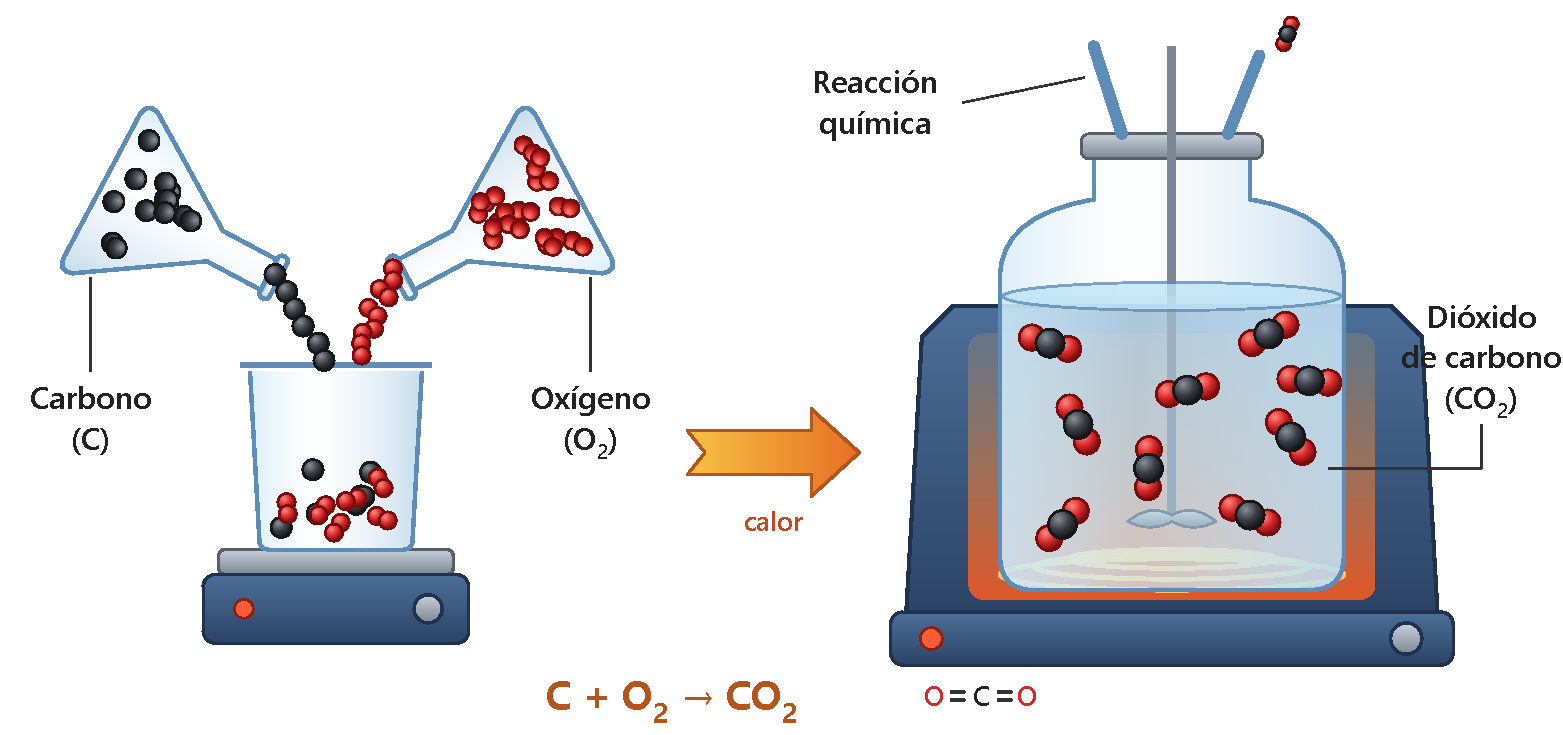
\includegraphics[width=\textwidth]{Figuras_SVG_ES/pdf/U8_reaccion_carbono_oxigeno.pdf}
    \caption{Reacción química}
    \label{fig:reaccion_quimica}
\end{figure}

\subsection{Cómo leer una reacción química}

Es necesario saber cómo escribir una reacción química a partir de su descripción con palabras.
Para ello seguimos las siguientes reglas.
Imaginemos la siguiente reacción general:
\begin{reaction*}
    A \gas{} + B \sld{} -> C \lqd{} + D \aq{}
\end{reaction*}
Aquí, los reactivos son A y B, mientras que los productos son C y D.
\begin{enumerate}[label=\numberballmDarkTeal]
        \item Si los reactivos o compuestos están escritos con su nombre, primero debemos obtener su fórmula.
        \item Si aparece el símbolo \( + \) en los reactivos, se lee como "reacciona con". Por ejemplo, en la ecuación anterior podemos decir que A reacciona con B.
        \item El símbolo \( \rightarrow \) se lee como \textquote{para formar} o \textquote{para dar}.
        \item Si el símbolo \( + \) está en los productos, ese \( + \) se lee como \textquote{y}.
        En el caso anterior podemos decir que se obtienen C \textquote{y} D.
        \item Junto a A aparece \gas{}, junto a B aparece \sld{}, junto a C aparece \lqd{}, mientras que junto a D aparece \aq{}. Estas palabras indican el estado de la materia de cada compuesto y tienen el siguiente significado:
        \begin{itemize}
            \item \sld{}: sólido.
            \item \lqd{}: líquido.
            \item \gas{}: gas.
            \item \aq{}: acuoso
        \end{itemize}
\end{enumerate}

\subsection{Cómo ocurre una reacción química}

Para que ocurra una reacción química, se deben seguir los siguientes pasos:
\begin{enumerate}[label=\numberballmDarkTeal]
        \item Los átomos de las moléculas reactivas deben separarse.
        \item Una vez separados los átomos, estos colisionan entre sí.
        Según la \negsubro{teoría de colisiones}, las reacciones químicas ocurren debido a colisiones entre átomos.
        Para que una colisión sea eficaz y produzca una reacción química, se debe cumplir lo siguiente:
        \begin{itemize}
            \item Los reactivos deben tener suficiente energía.
            \item Los reactivos deben colisionar con la orientación adecuada.
        \end{itemize}
        \item Una vez que ocurre una colisión eficaz, se obtienen los productos correspondientes.

        \begin{figure}[H]
            \centering
%            \includegraphics[scale=0.18]{images/reacciones_quimicas/reaccion_quimica_proceso_gemini}
            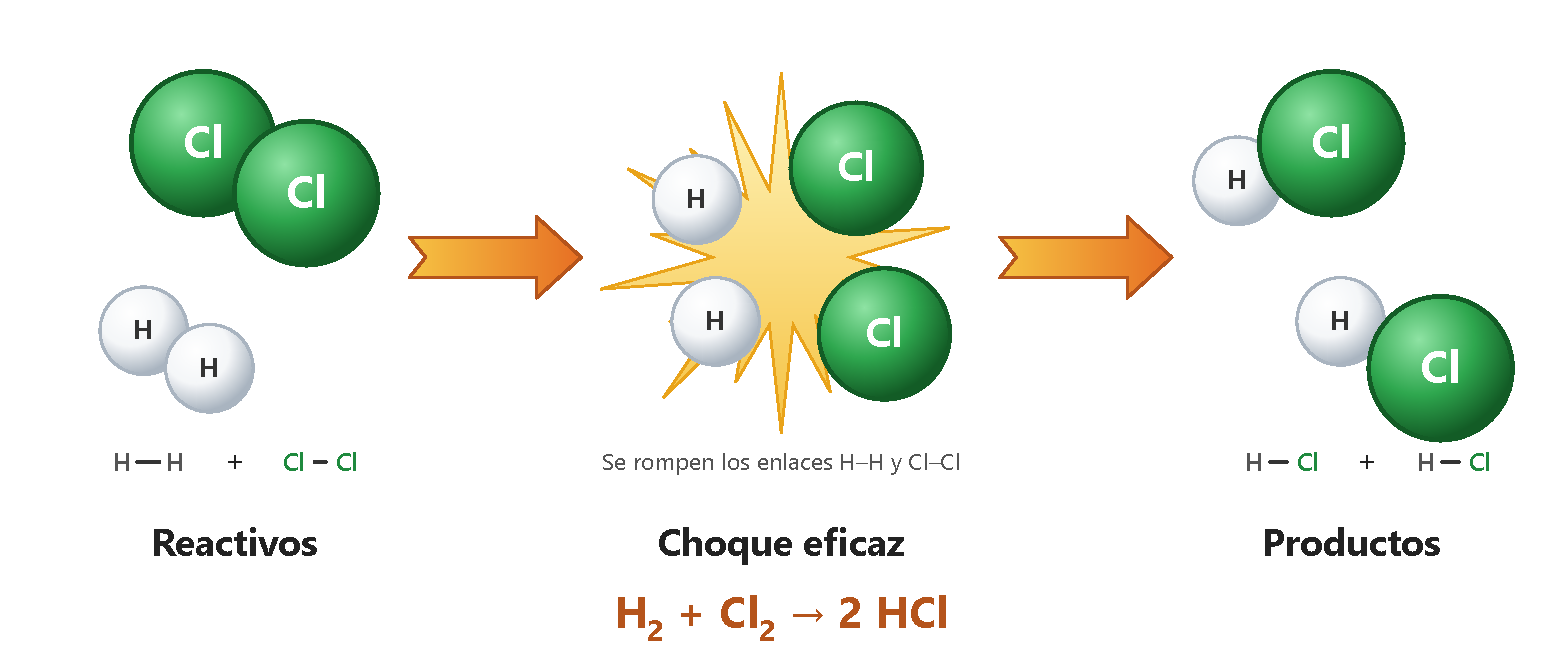
\includegraphics[width=0.95\textwidth]{Figuras_SVG_ES/pdf/U8_reaccion_proceso_H2_Cl2.pdf}
            \caption{}
            \label{fig:reaccion_quimica_proceso}
        \end{figure}
\end{enumerate}

%        Página xxx. Ejercicios 2 y 3.
%        \begin{exercise}{}
%            \begin{solu}{\arabic{ejercicionumero}}
%            \end{solu}
%        \end{exercise}

\begin{exercise}
    Cu representa el elemento cobre, S el elemento azufre y CuS el sulfuro de cobre(II). Usa tus propias palabras para explicar qué representa esta
    ecuación química
    \begin{solu}{\arabic{ejercicionumero}}
        Cu representa el elemento cobre, S el elemento azufre y CuS el sulfuro de cobre(II). Usa tus propias palabras para explicar qué representa esta
    ecuación química:

        El azufre reacciona con el cobre para formar sulfuro
        de cobre (II). En concreto, un átomo de azufre reacciona con un
        átomo de cobre para formar sulfuro de cobre (II).
    \end{solu}
\end{exercise}

\begin{exercise}
    El carbonato de calcio (CaCO3) se descompone a
    altas temperaturas en óxido de calcio (CaO) y
    dióxido de carbono (CO2). Este proceso se conoce como
    calcinación. Escribe la ecuación química para esta
    reacción.
    \begin{solu}{\arabic{ejercicionumero}}
         El carbonato de calcio (CaCO3) se descompone a altas temperaturas en óxido de calcio (CaO) y dióxido de carbono (CO2). Este proceso se conoce como calcinación. Escribe la ecuación química para esta reacción.

        \begin{reaction*}
            CaCO3\sld{} → CaO\sld{} + CO2\gas{}
        \end{reaction*}
    \end{solu}
\end{exercise}

\begin{exercise}
    ¿Cómo se llama la teoría que explica cómo ocurren las reacciones químicas?
    \begin{solu}{\arabic{ejercicionumero}}
         ¿Cómo se llama la teoría que explica cómo ocurren las reacciones químicas?

        Teoría de colisiones
    \end{solu}
\end{exercise}

\begin{exercise}
    Explica con palabras las siguientes ecuaciones químicas:
    \begin{reaction*}
        CuCO3\sld{} -> CUO\sld{} + CO2\gas{}
    \end{reaction*}
    \begin{reaction*}
        H2\gas{} + O2\gas{} ->  H2O\lqd{}
    \end{reaction*}
    \begin{solu}
         Explica con palabras las siguientes ecuaciones químicas:
    \begin{reaction*}
        CuCO3\sld{} -> CUO\sld{} + CO2\gas{}
    \end{reaction*}
    \begin{reaction*}
        H2\gas{} + O2\gas{} ->  H2O\lqd{}
    \end{reaction*}


        El carbonato de cobre (II) se descompone al calentarse
        para dar óxido de cobre (II) sólido y dióxido de
        carbono gaseoso.
        El hidrógeno gaseoso reacciona con oxígeno gaseoso
        para formar agua en estado líquido. En concreto, dos
        moléculas de hidrógeno reaccionan con una molécula de
        oxígeno para dar
        dos moléculas de agua.
        El ácido clorhídrico acuoso reacciona con hidróxido
        de sodio acuoso para dar cloruro de sodio acuoso
        y agua.
    \end{solu}
\end{exercise}


\section{Principio de Lavoisier. Ley de conservación de la masa}

En una reacción química (en un recipiente cerrado) la suma de las masas de los reactivos debe ser igual a la suma de las masas de los productos, es decir, \negsubro{la masa se conserva}.

Consideremos la siguiente reacción:
\begin{reaction*}
    AgNO3 + HCl -> AgCl + HNO3
\end{reaction*}
Si tenemos \qty{17}{\g} de \ch{AgNO3} y reacciona con \qty{3.65}{\g} de \ch{HCl}, se formarán \qty{14.35}{\g} de \ch{AgCl} y \qty{6.3}{\g} de \ch{HNO3}.
\begin{figure}[H]
    \centering
%    \includegraphics[scale=0.2]{images/reacciones_quimicas/conservacion_masa_EN}
    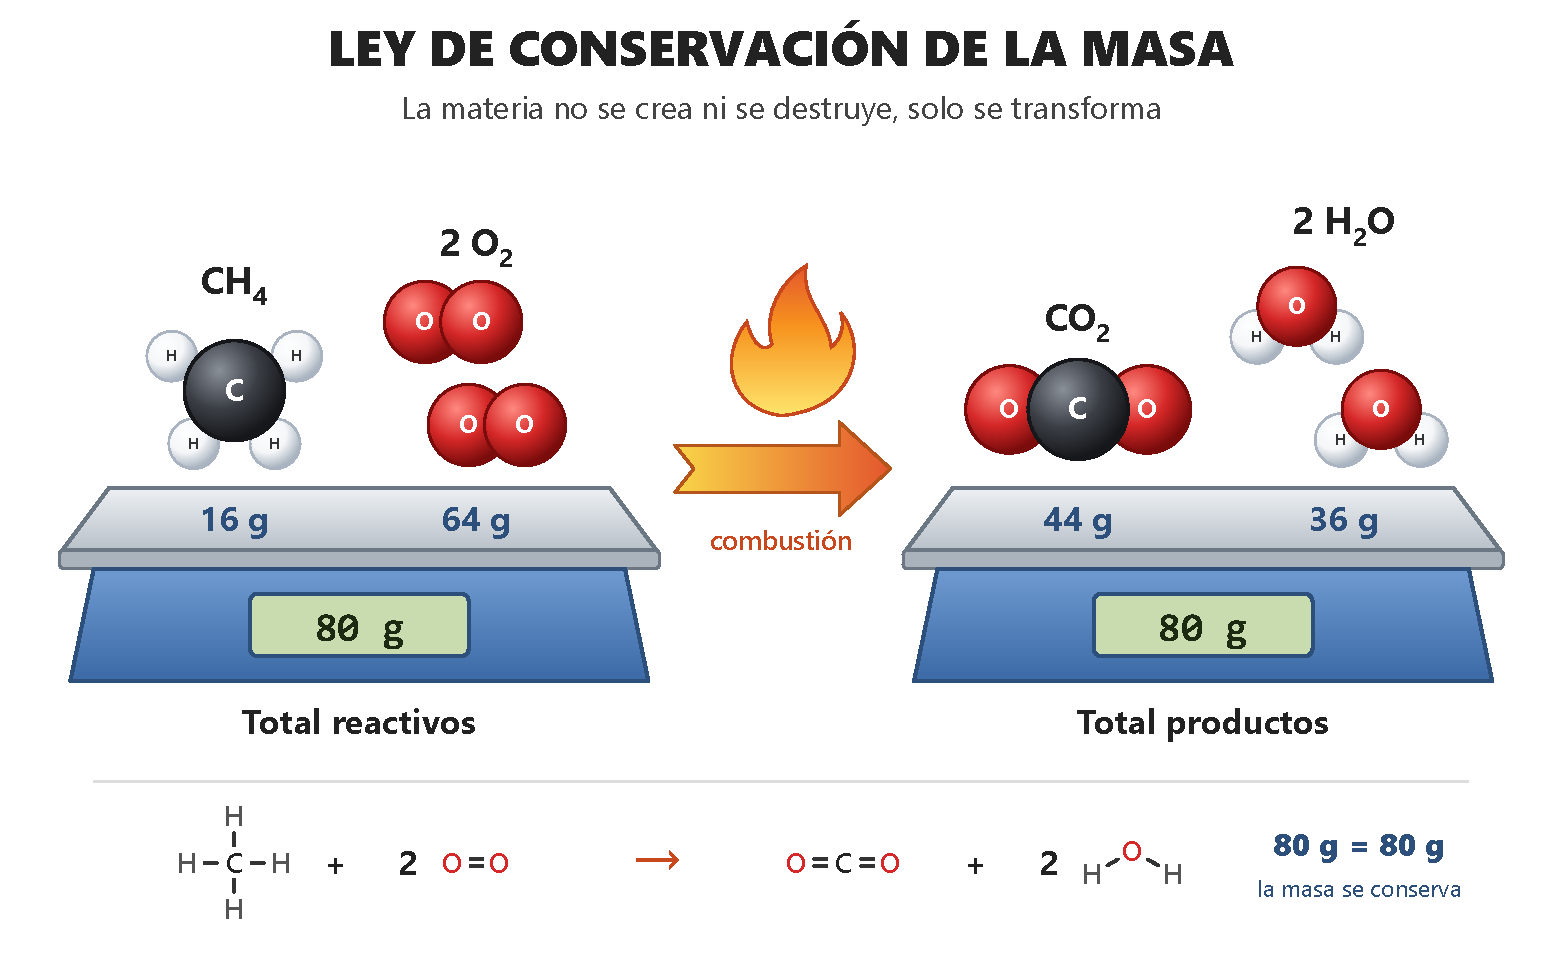
\includegraphics[width=0.9\textwidth]{Figuras_SVG_ES/pdf/U8_conservacion_masa.pdf}
    \caption{Ley de conservación de la masa}
    \label{fig:conservacion_masa}
\end{figure}

\subsection{Las reacciones químicas y la ley de conservación de la masa}

Toda reacción química debe cumplir el principio de Lavoisier y, por lo tanto:

\begin{displayquote}
    Debemos tener el mismo número de átomos de cada elemento en los reactivos (lado izquierdo) y en los productos (lado derecho).
    Cuando se da esta situación decimos que la reacción está \textbf{ajustada}
\end{displayquote}

Si la reacción química no está ajustada, debemos ajustarla para que se cumpla el principio de Lavoisier.

Los números colocados delante de cada fórmula química se conocen como \negsubro{coeficientes estequiométricos}.
\vspace*{12pt}
%
%    \begin{equation*}
%        \eqnmarkbox[blue]{hidrogeno}{\ch{2}}
%        \ch{H2 + }
%        \eqnmarkbox[violet]{oxigeno}{\ch{1}}
%        \ch{O2 ->}
%        \eqnmarkbox[red]{agua}{\ch{2}}
%        \ch{H2O}
%    \end{equation*}
%
%    \annotate[yshift=-2em]{below}{hidrogeno}{Coef. estequiométrico del \ch{H2}}
%    \annotate[yshift=-3.5em]{below}{oxigeno}{Coef. estequiométrico del \ch{O2}}
%    \annotate[yshift=-2em]{below}{agua}{Coef. estequiométrico del \ch{H2O}}
%
%\annotate[yshift=1em]{left}{node1}{Presión}
%    \annotate[yshift=-0.5em]{below,left}{volumen}{Volumen}
%    \annotate[yshift=1em]{}{moles}{número de moles}
%    \annotate[yshift=-2em]{below,left}{constante}{Constante de los gases ideales}
%    \annotate[yshift=-1em]{below}{temperatura}{Temperatura}
%
\begin{centeredequation}
    \eqnmarkbox[blue]{coehidrogeno}{\ch{2}}
    \tikzmarknode{reaccion}{\ch{H2 + O2 ->}}
    \eqnmarkbox[red]{coeagua}{\ch{2}}
    \ch{H2O}
\end{centeredequation}
%\begin{equation*}
%    \eqnmarkbox[blue]{coehidrogeno}{\ch{2}}
%    \tikzmarknode{reaccion}{\ch{H2 + O2 ->}}
%    \eqnmarkbox[red]{coeagua}{\ch{2}}
%    \ch{H2O}
%    %\tikzmarknode{node4}{\ch{H2O}}
%\end{equation*}
\vspace{8pt}
\annotate[yshift=1em]{}{coehidrogeno,coeagua}{Coeficientes estequiométricos}

%    \begin{figure}[H]
%        \centering
%        \includegraphics[scale=1]{images/unidad_5_imagenes/coeficientes_estequiometricos}
%        \caption{}
%        \label{fig:stechiometric_coefficients}
%    \end{figure}
Estos coeficientes estequiométricos nos indican el número de moléculas o moles de cada compuesto que reaccionan entre sí para obtener el número correspondiente de moléculas o moles de productos.

%    Por ejemplo, sea la reacción:
%    \begin{reaction*}
%        2 H2 + O2 -> 2 H2O
%    \end{reaction*}

%    Como podemos ver está ajustada.
Estos coeficientes estequiométricos nos indican que:
\begin{itemize}
    \item \negsubro{¡¡¡¡IMPORTANTE!!!!}: no aparece ningún número delante de \ch{O2}, cuando no tenemos un número debemos suponer que es un \( 1 \). Esto significa que reaccionará 1 mol de \ch{O2}.
    \item 2 moléculas de hidrógeno (\ch{H2}) reaccionan con 1 molécula de oxígeno (\ch{O2}) para formar 2 moléculas de agua (\ch{H2O}).
    \item 2 moles de hidrógeno (\ch{H2}) reaccionan con 1 mol de oxígeno (\ch{O2}) para formar 2 moles de agua (\ch{H2O}).
    \item Estos coeficientes también nos indican que 2 moles de \ch{H2} están relacionados con 1 mol de \ch{O2} y a su vez con 2 moles de \ch{H2O}.

\end{itemize}

\subsection{Pasos para el ajuste (Método de tanteo)}

\begin{enumerate}
    \item \textbf{Contar:} Contar los átomos de cada elemento en ambos lados de la flecha.
    \item \textbf{Ajustar con coeficientes:} Colocar números grandes delante de las moléculas para multiplicar el número de átomos.
    \item \textbf{Orden recomendado:}
    \begin{itemize}
        \item Metales y no metales.
        \item Hidrógeno ($H$).
        \item Oxígeno ($O$).
    \end{itemize}
\end{enumerate}

\paragraph{Ejemplo paso a paso: combustión del metano}

Queremos ajustar la siguiente reacción:
\[ \ch{CH4 + O2 -> CO2 + H2O} \]

        {\noindent  \textbf{Paso 1: Contar los átomos iniciales}}

\begin{itemize}
    \item Reactivos: $C=1, H=4, O=2$
    \item Productos: $C=1, H=2, O=3$ (2 del \ch{CO2} y 1 del \ch{H2O})
\end{itemize}

        {\noindent \textbf{Paso 2: Ajustar el hidrógeno}}

Como hay 4 $H$ en el lado izquierdo y solo 2 en el derecho, colocamos un \textbf{2} delante del agua:
\[ \ch{CH4 + O2 -> CO2 + 2 H2O} \]
Ahora tenemos: $H = 2 \times 2 = 4$. ¡Ajustado!

        {\noindent \textbf{Paso 3: Ajustar el oxígeno}}

Ahora en el lado derecho hay: 2 (del \ch{CO2}) + 2 (de \ch{2 H2O}) = 4 átomos de $O$.
En el lado izquierdo solo hay 2. Colocamos un \textbf{2} delante de \ch{O2}:
\[ \ch{CH4 + 2 O2 -> CO2 + 2 H2O} \]

        {\noindent \textbf{Resultado final}} La ecuación ajustada es:
\[ \mathbf{\ch{CH4 + 2 O2 -> CO2 + 2 H2O}} \]


\begin{exercise}
    En tu cuaderno, ajusta las ecuaciones químicas.
    \begin{multicols}{2}
        \begin{enumerate}[label=\letraminuscula]
            \item
            \begin{reaction*}
                Na\sld{} + O2\gas{}  → Na2O2\sld{}
            \end{reaction*}
            \item
            \begin{reaction*}
                H2 \gas{} + Cl2\gas{} → HCl\gas{}
            \end{reaction*}
            \item
            \begin{reaction*}
                Ca\sld{} + O2\gas{} → CaO\sld{}
            \end{reaction*}
            \item
            \begin{reaction*}
                Al\sld{} + Br2\lqd{} → AlBr3\sld{}
            \end{reaction*}
        \end{enumerate}
    \end{multicols}
    \begin{solu}
        \begin{enumerate}[label=\letraminuscula]
            \item
            \begin{reaction*}
                4 Na(s) + 2 O2(g) → 2 Na2O2(s)
            \end{reaction*}
            \item
            \begin{reaction*}
                2 H2(g) + 2 Cl2(g) → 4 HCl(g)
            \end{reaction*}
            \item
            \begin{reaction*}
                2 Ca(s) + O2(g) → 2 CaO(s)
            \end{reaction*}
            \item
            \begin{reaction*}
                2 Al(s) + 3 Br2(l) → 2 AlBr3(s)
            \end{reaction*}
        \end{enumerate}
    \end{solu}
\end{exercise}

\begin{exercise}
    Explica cómo se ajustan las ecuaciones químicas
    %\marcador{interesante para explicar como se ajustan las reacciones químicas.}
    \begin{solu}
        ¿Cómo ajustamos las ecuaciones químicas? Primero,
        identificamos los reactivos, las sustancias del
        lado izquierdo de la ecuación, y los productos, las
        sustancias del lado derecho de la ecuación.
        Después, contamos el número total de átomos de cada
        elemento en ambos lados de la ecuación. Si no son
        iguales en ambos lados entonces la ecuación no está
        ajustada.
        Para ajustar una ecuación química solo podemos cambiar
        los coeficientes. Los subíndices no se pueden cambiar.
        Después de haber cambiado los coeficientes, para ajustar
        tu ecuación cuenta de nuevo el número total de átomos de
        cada elemento y asegúrate de que el número total en
        ambos lados es igual. Si lo es, ahora tienes
        una ecuación química ajustada.
        a. Para ajustar una ecuación química, podemos cambiar
        el coeficiente pero nunca los subíndices.
        b. Tendremos una ecuación ajustada si el número
        total de átomos de un elemento dado es el
        mismo en ambos lados de la ecuación.
    \end{solu}
\end{exercise}

\begin{exercise}
    El hidrógeno reacciona con el oxígeno para dar agua. ¿Qué masa de agua líquida se obtiene si \qty{2}{\g} de hidrógeno reacciona exactamente con \qty{16}{\g} de oxígeno?
    \begin{solu}
        A partir de la ley de conservación de la masa, sabemos que se formarán \qty{18}{\g} de agua.
    \end{solu}
\end{exercise}

\begin{exercise}
    Hacemos reaccionar hierro con azufre para obtener sulfuro de hierro:
    \begin{reaction*}
        S (s) + Fe (s) → FeS (s)
    \end{reaction*}
    Sabemos que 32 g de azufre reaccionan exactamente con
    56 g de hierro.
    \begin{enumerate}[label=\letraminuscula]
            \item ¿Qué masa de sulfuro de hierro se obtiene?
            \item ¿Cuál es el porcentaje de azufre y hierro en el
            sulfuro de hierro?
    \end{enumerate}
    \begin{solu}
        \begin{enumerate}[label=\letraminuscula]
                \item Si reaccionan las masas exactas del enunciado,
                producirán 32 g + 56 g = 88 g de sulfuro
                de hierro.
                \item 32 g de S / 88 g de FeS = 36,36\% de S
                56 g de Fe / 88 g de FeS = 63,64\% de Fe
        \end{enumerate}
    \end{solu}
\end{exercise}

\begin{exercise}
    En un experimento, comprobamos que 3,2 g de azufre
    (S) reacciona completamente con 20 g de mercurio (Hg) para dar
    sulfuro de mercurio (II) (HgS). Ajusta la reacción
    y realiza los cálculos para las preguntas siguientes.
    \begin{reaction*}
        S (s) + Hg (l) → HgS (s)
    \end{reaction*}
    \begin{enumerate}[label=\letraminuscula]
            \item la cantidad de sulfuro de mercurio obtenida.
            \item la masa de azufre necesaria para reaccionar completamente con
            5 g de mercurio.
            \item la masa de mercurio necesaria para reaccionar completamente con
            10 g de azufre.
            \item el porcentaje de azufre y mercurio en el
            sulfuro de mercurio (II).
    \end{enumerate}
    \begin{solu}{\arabic{ejercicionumero}}

        \begin{enumerate}[label=\letraminuscula]
                \item Si reaccionan las masas exactas del enunciado,
                producirán 3,2 g + 20 g = 23,2 g de sulfuro
                de hierro.
                \item A partir de la relación entre las masas
                de azufre y mercurio que reaccionan para formar
                sulfuro de mercurio, la masa debe ser:
                3,2 g de S / 20 g de Hg = x g de S / 5 g de Hg;
                x = 0,8 g de S
                \item 3,2 g de S / 20 g de Hg = 10 g de S / x g de Hg;
                x = 62,5 g de Hg
                \item 3,2 g de S / 23,2 g de HgS = 13,8\% de S
                20 g de Hg / 23,2 g de HgS = 86,2\% de Hg
        \end{enumerate}
    \end{solu}
\end{exercise}

\begin{exercise}
    Escribe la ecuación química de la reacción del
    magnesio sólido con cloruro de hidrógeno (HCl)
    en disolución acuosa para dar cloruro de magnesio
    sólido (MgCl2) e hidrógeno gaseoso (H2). Ajusta
    la ecuación química.
    \begin{solu}

        La reacción es la siguiente:

        Mg (s) + HCl (aq) → MgCl2 (s) + H2 (g)
        2 Mg (s) + 2 HCl (aq) → 2 MgCl2 (s) + H2 (g)
    \end{solu}
\end{exercise}

\begin{exercise}
    Ajusta estas reacciones.
    \begin{enumerate}[label=\letraminuscula]
            \item Ca (s) + O2 (g) → CaO (s)
            \item CuO (s) + C (s) → Cu (s) + CO2 (g)
            \item Na (s) + Cl2 (g) → NaCl (s)
            \item Al (s) + O2 (g) → Al2O3 (s)
            \item Fe (s) + O2 (g) → FeO (s)
    \end{enumerate}
    \begin{solu}
        \begin{enumerate}[label=\letraminuscula]
                \item 2 Ca (s) + O2 (g) → 2 CaO (s)
                \item 2 CuO (s) + C (s) → 2 Cu (s) + CO2 (g)
                \item 2 Na (s) + Cl2 (g) → 2 NaCl (s)
                \item 4 Al (s) + 3 O2 (g) → 2 Al2O3 (s)
                \item 2 Fe (s) + O2 (g) → 2 FeO (s)a
        \end{enumerate}
    \end{solu}
\end{exercise}


\section{Cálculos con reacciones químicas}

Los cálculos en reacciones químicas nos permitirán saber qué cantidad (ya sea en gramos o moles) de productos se obtendrá o qué cantidad de reactivos necesitaremos.
Como ejemplo utilizaremos la reacción: el hidrógeno reacciona con el oxígeno para formar agua.

Para realizar los cálculos correctamente, se deben seguir los siguientes pasos:
\begin{enumerate}[label=\numberballmDarkTeal]
        \item Identificar los reactivos y productos.
        En este caso los reactivos serán \ch{H2} y \ch{O2} mientras que tendremos un único producto que es \ch{H2O}.
        \item Si en la reacción dicen hidrógeno, nitrógeno, oxígeno, flúor, cloro, bromo o yodo, siempre los escribiremos como \ch{H2}, \ch{N2}, \ch{O2}, \ch{F2}, \ch{Cl2}, \ch{Br2}, o \ch{I2}.
        También pueden nombrarse como nitrógeno molecular o dinitrógeno.
        Para el resto de los elementos mencionados anteriormente es lo mismo.
        \item Escribir la reacción química utilizando sus fórmulas químicas correspondientes.
        \begin{reaction*}
            H2 + O2 -> H2O
        \end{reaction*}
        \item Ajustar la reacción química si es necesario.
        \begin{reaction*}
            2 H2 + O2 -> 2 H2O
        \end{reaction*}
        \item Si nos dan cantidades en gramos, debemos convertirlas todas a moles (representaremos los moles con la letra \( \bm{n} \)).
        Si nos dan por ejemplo \qty{10}{\g} de \ch{H2O}, tendríamos que calcular primero la masa molar del agua que en este caso es \qty{18}{\g\per\mol}
        \begin{itemize}
            \item Usando la fórmula:
            \begin{equation*}
                n_{\ch{H2O}} = \dfrac{\text{gramos de sustancia}}{\text{masa molar del compuesto}} = \dfrac{\qty{10}{\g}}{\qty{18}{\g\per\mol}} = \qty{0.56}{\mol}\ \text{de \ch{H2O}}
            \end{equation*}
            \item También podemos usar factores de conversión:
            \begin{equation*}
                10\ \cancelred{\unit{\g}\ \text{de \ch{H2O}}} \cdot \dfrac{\qty{1}{\mol}\ \text{de \ch{H2O}}}{18\ \cancelred{\unit{\g} \ \text{de \ch{H2O}}}} = \qty{0.56}{\mol}\ \text{de \ch{H2O}}
            \end{equation*}
        \end{itemize}
        \item Ahora calculamos los moles necesarios para el resto de los compuestos utilizando los coeficientes estequiométricos.
        Ahora calcularemos los moles de \ch{H2} y \ch{O2}:

        Cálculo de los moles de \ch{H2}
        \begin{equation*}
            0.56\ \cancelred{\unit{\mol}\ \text{de \ch{H2O}}} \cdot \dfrac{\qty{2}{\mol}\ \text{de \ch{H2}}}{1\ \cancelred{\unit{\mol} \ \text{de \ch{H2O}}}} = \qty{1.12}{\mol}\ \text{de \ch{H2}}
        \end{equation*}
        Cálculo de los moles de \ch{O2}
        \begin{equation*}
            0.56\ \cancelred{\unit{\mol}\ \text{de \ch{H2O}}} \cdot \dfrac{\qty{1}{\mol}\ \text{de \ch{O2}}}{2\ \cancelred{\unit{\mol} \ \text{de \ch{H2O}}}} = \qty{0.28}{\mol}\ \text{de \ch{O2}}
        \end{equation*}
        \item Ahora calculamos en gramos las cantidades de todos esos compuestos solicitados

        Imaginemos ahora que calculamos la cantidad en gramos de \ch{H2} y \ch{O2}.
        Para ello usaremos los moles calculados anteriormente y la masa molar de cada compuesto.

        Cálculo de las masas molares:
        \begin{itemize}
            \item \ch{H2}: \( 2 \times 1 \text{ uma} = \qty{2}{\uma} =  \qty{2}{\g\per\mol} \)
            \item \ch{O2}: \( 2 \times 16 \text{ uma} = \qty{32}{\uma} = \qty{32}{\g\per\mol} \)
        \end{itemize}

        Ahora realizamos los cálculos que mencionamos anteriormente, lo haremos de dos formas distintas (solo es necesaria una) usando la fórmula de los moles y factores de conversión.
        \begin{itemize}
            \item Cálculo de los gramos de \ch{H2} y \ch{O2} usando la fórmula:

            Sabemos que \( n = \dfrac{\text{gramos de compuesto}}{\text{masa molar del compuesto}} \)

            si despejamos los gramos del compuesto tendremos:

            \( \text{gramos de compuesto} = n\cdot \text{masa molar del compuesto} \)

            gramos de \ch{H2} = \( 1.12 \cdot 2 = \qty{2.24}{\g}\ \text{de \ch{H2}} \).

            gramos de \ch{O2} = \( 0.28 \cdot 32 = \qty{8.96}{\g}\ \text{de \ch{O2}} \).
            \item Cálculo de los gramos de \ch{H2} y \ch{O2} usando factores de conversión. Para esto partiremos ahora de los moles obtenidos de \ch{H2} y \ch{O2} calculados en el apartado anterior y usando las masas molares de cada compuesto.

            \textbf{Cantidad de \ch{H2}}:
            \begin{equation*}
                1.12\ \cancelred{\unit{\mol}\ \text{de \ch{H2}}} \cdot \dfrac{\qty{2}{\g}\ \text{de \ch{H2}}}{1\ \cancelred{\unit{\mol} \ \text{de \ch{H2}}}} = \qty{2.24}{\g}\ \text{de \ch{H2}}
            \end{equation*}

            \textbf{Cantidad de \ch{O2}}:
            \begin{equation*}
                0.28\ \cancelred{\unit{\mol}\ \text{de \ch{O2}}} \cdot \dfrac{\qty{32}{\g}\ \text{de \ch{H2}}}{1\ \cancelred{\unit{\mol} \ \text{de \ch{O2}}}} = \qty{0.96}{\g}\ \text{de \ch{HO}}
            \end{equation*}
        \end{itemize}
\end{enumerate}

\begin{example}

    Dos elementos como el azufre y el cobre reaccionan para formar sulfuro de cobre(II). ¿Qué masa de sulfuro de cobre(II) se obtiene si partimos de \qty{64}{\g} de azufre?
    ¿Qué cantidad en gramos de cobre necesitamos?

    \begin{enumerate}[label=\numberballmDarkTeal]
            \item Identificamos los reactivos y productos.
            En este caso, los reactivos son \ch{S} y \ch{Cu} mientras que el producto es \ch{CuS}.
            \item Escribimos la reacción química:
            \begin{reaction*}
                S + Cu -> Cu2S
            \end{reaction*}
            \item Ajustamos la reacción y sería:
            \begin{reaction*}
                S + 2 Cu -> Cu2S
            \end{reaction*}
            \item Ahora calculamos los moles de todas las cantidades que pide el ejercicio.
            \begin{equation*}
                64\ \cancelred{\unit{\g}\ \text{de \ch{S}}} \cdot \dfrac{\qty{1}{\mole}\ \text{de \ch{S}}}{32\ \cancelred{\unit{\g} \ \text{de \ch{S}}}} = \qty{2}{\mol}\ \text{de \ch{S}}
            \end{equation*}
            \item Como piden la cantidad de \ch{CuS} y \ch{Cu}, calculamos los moles de cada especie con cálculos estequiométricos.
            \begin{itemize}
                \item Para CuS:
                \begin{equation*}
                    2\ \cancelred{\unit{\mol}\ \text{de \ch{S}}} \cdot \dfrac{\qty{1}{\mole}\ \text{de \ch{CuS}}}{1\ \cancelred{\unit{\mole} \ \text{de \ch{S}}}} = \qty{2}{\mol}\ \text{de \ch{S}}
                \end{equation*}
                \item Para Cu:
                \begin{equation*}
                    2\ \cancelred{\unit{\mol}\ \text{de \ch{S}}} \cdot \dfrac{\qty{2}{\mole}\ \text{de \ch{Cu}}}{1\ \cancelred{\unit{\mole} \ \text{de \ch{S}}}} = \qty{4}{\mol}\ \text{de \ch{S}}
                \end{equation*}
            \end{itemize}
            \item Ahora calculamos las masas en gramos de cada especie solicitada.
            \begin{itemize}
                \item Para CuS:
                \begin{equation*}
                    2\ \cancelred{\unit{\mol}\ \text{de \ch{CuS}}} \cdot \dfrac{\qty{95.5}{\g}\ \text{de \ch{CuS}}}{1\ \cancelred{\unit{\mole} \ \text{de \ch{CuS}}}} = \qty{191}{\g}\ \text{de \ch{CuS}}
                \end{equation*}
                \item Para Cu:
                \begin{equation*}
                    4\ \cancelred{\unit{\mol}\ \text{de \ch{Cu}}} \cdot \dfrac{\qty{63.5}{\g}\ \text{de \ch{Cu}}}{1\ \cancelred{\unit{\mole} \ \text{de \ch{Cu}}}} = \qty{254}{\g}\ \text{de \ch{Cu}}
                \end{equation*}
            \end{itemize}
            Estos mismos cálculos se pueden hacer utilizando la fórmula
            \begin{equation*}
                n = \dfrac{\text{gramos}}{\text{masa molar}} \longrightarrow \text{gramos} = n \cdot \text{masa molar}
            \end{equation*}
            \begin{itemize}
                \item Para CuS:
                \begin{equation*}
                    \text{gramos de } \ch{CuS} = 2\cdot 95.5 = \qty{191}{\g}\ \text{de \ch{CuS}}
                \end{equation*}
                \item Para CuS:
                \begin{equation*}
                    \text{gramos de } \ch{Cu} = 4\cdot 63.5 = \qty{254}{\g}\ \text{de \ch{Cu}}
                \end{equation*}
            \end{itemize}
    \end{enumerate}
\end{example}



\begin{exercise}
    ¿Qué masa de hidrógeno se forma cuando 27 g de aluminio reaccionan con exceso de ácido clorhídrico (HCl) según la ecuación?
    \begin{reaction*}
        2 Al + 6 HCl → 2 AlCl3 + 3 H2
    \end{reaction*}

    \begin{solu}
        \qty{3}{\g}
    \end{solu}
\end{exercise}

\begin{exercise}
    El carbonato de calcio (CaCO3), o piedra caliza,
    se descompone a altas temperaturas en óxido
    de calcio (CaO), o cal, y dióxido de carbono,
    según esta ecuación:
    \begin{reaction*}
        CaCO3 (s) → CaO (s) + CO2 (g)
    \end{reaction*}
    Si calentamos 160 kg de carbonato de calcio,
    obtenemos 89,6 kg de óxido de calcio. ¿Qué masa de
    óxido de calcio obtendríamos a partir de 80 kg de
    carbonato?
    \begin{solu}
        \qty{44.8}{\kg}
    \end{solu}
\end{exercise}

\begin{exercise}
    Al calentar 0,5 g de hierro pulverizado bajo una corriente
    de cloro gaseoso se produce dicloruro de hierro
    según esta reacción:
    \begin{reaction*}
        Fe (s) + Cl2 (g) → FeCl2 (s)
    \end{reaction*}
    \begin{enumerate}[label=\letraminuscula]
        \item Calcula la masa de cloro consumida.
        \item Calcula la masa de dicloruro de hierro
        producida.
    \end{enumerate}
    \begin{solu}
        \begin{enumerate}[label=\letraminuscula]
            \item 0,64 g
            \item 1,14 g
        \end{enumerate}
    \end{solu}
\end{exercise}

\begin{exercise}
    Un gramo de cinc arde en el aire según la ecuación:
    \begin{reaction*}
        Zn (s) + O2 (g) → ZnO (s)
    \end{reaction*}
    \begin{enumerate}[label=\letraminuscula]
        \item Ajusta la ecuación química.
        \item ¿Cuánto oxígeno consume?
        \item ¿Cuánto óxido de cinc produce?
        \item ¿Qué porcentaje de óxido de cinc es cinc?
        \item ¿Se cumple la ley de conservación de la masa?
    \end{enumerate}
    \begin{solu}
        \begin{enumerate}[label=\letraminuscula]
            \item \begin{reaction*}
                      2 Zn (s) + O2 (g) → 2 ZnO (s)
            \end{reaction*}
            donde \( \ch{Zn} = \qty{130.8}{\g}; \ch{O2} = \qty{32}{\g}; \ch{ZnO} = \qty{162.8}{\g} \)
        \end{enumerate}
    \end{solu}
\end{exercise}

\begin{exercise}
    El mercurio y el azufre reaccionan para formar sulfuro de mercurio según esta fórmula:
    \begin{reaction*}
        S (s) + Hg (s) → HgS (s)
    \end{reaction*}
    Si reaccionan 20 g de Hg:
    \begin{enumerate}[label=\letraminuscula]
        \item ¿con cuánto azufre reacciona?
        \item ¿qué masa de sulfuro de mercurio
        produce?
    \end{enumerate}
    \begin{solu}

    \end{solu}
\end{exercise}

\begin{exercise}
    El magnesio (Mg) reacciona con oxígeno (O2) para dar óxido de magnesio (MgO).
    \begin{enumerate}[label=\letraminuscula]
        \item Escribe y ajusta esta ecuación química.
        \item Si 48,6 g de magnesio reaccionan con la
        cantidad necesaria de oxígeno, ¿cuánto
        óxido de magnesio se obtiene?
    \end{enumerate}
    \begin{solu}
        \begin{enumerate}[label=\letraminuscula]
            \item La ecuación ajustada es:
            \begin{reaction*}
                2Mg + O2 → 2MgO
            \end{reaction*}
            \item Escribimos la reacción y las masas involucradas:
            \begin{reaction*}
                2 Mg + O2 → 2 MgO
            \end{reaction*}
            \( \ch{Mg} = \qty{48.6}{\g}; \ch{O2} = \qty{32}{\g}; \ch{MgO} = \qty{80.6}{\g} \)

            Obtendríamos 80,6 g de MgO.
        \end{enumerate}
    \end{solu}
\end{exercise}


%
%    \section{Ideal Gas Law}
%
%    In a chemical reaction, it is advisable to know the state too atter to the compound, that is, whether it is a solid, a gas, or a liquid.
%    To indicate it in the chemical reaction, \gas{} is placed next to the compound for gases, \lqd{} and \sld{} for a solid.
%    An example could be:
%
%    \begin{reaction*}
%        O2\gas{} + C \sld{} -> CO2 \lqd{}
%    \end{reaction*}
%
%    For gases, the three gas laws (Gay-Lussac's Law, Charles's Law, and Boyle-Mariotte's Law) can be concentrated into one law known as the \textbf{Ideal Gas Law} and this law relates the magnitudes too ressure, volume, and temperature with the amount to substance expressed in moles.
%    The mathematical expression to this law will be:
%    \vspace{20pt}
%
%    \begin{equation*}
%        \eqnmarkbox[blue]{presion}{p}
%        \cdot
%        \eqnmarkbox[red]{volumen}{V}
%        =
%        \eqnmarkbox[mDarkTeal]{moles}{n}
%        \cdot
%        \eqnmarkbox[orange]{constante}{R}
%        \cdot
%        \eqnmarkbox[violet]{temperatura}{T}
%    \end{equation*}
%    \vspace{25pt}
%    \annotate[yshift=1em]{left}{presion}{Pressure}
%    \annotate[yshift=-0.5em]{below,left}{volumen}{Volume}
%    \annotate[yshift=1em]{}{moles}{number to moles}
%    \annotate[yshift=-2em]{below,left}{constante}{Ideal gas constant}
%    \annotate[yshift=-1em]{below}{temperatura}{Temperature}
%
%    where:
%    \begin{itemize}
%        \item \( p \) is the system pressure expressed in \unit{\atmosphere}.
%        \item \( V \) is the system volume expressed in \unit{\litre}.
%        \item \( R \) is a constant called the ideal gas constant and has a value  \( R = \ctegases{} \).
%        \item \( T \) is the system temperature expressed in \unit{\kelvin}.
%    \end{itemize}

%
%        \begin{exercise}{}
%            Aluminium reacts with oxygen producing aluminium oxide.
%            Calculate the mass to aluminium oxide produced when \qty{15}{\g} to aluminium reacts with excess oxygen.
%        \end{exercise}
%
%        \begin{exercise}{}
%            What is the volume in mL occupied by an ideal gas if \qty{0.553}{\mol} are at a temperature to \qty{1226.49}{\kelvin} and a pressure to \qty{4935}{\mmHg}?
%        \end{exercise}
%
%        \begin{exercise}{}
%            What is the temperature in \unit{\kelvin} to an ideal gas, if \qty{0.405}{\mole} occupy a volume to \qty{7720}{\mL} at a pressure to \qty{790}{\mmHg}?
%        \end{exercise}
%
%        \begin{exercise}{}
%            What is the temperature in \unit{\degreeCelsius} to an ideal gas, if \qty{0.746}{\mol} occupy a volume to \qty{9890}{\mL} at a pressure to \qty{1.41}{\atmosphere}?
%        \end{exercise}
%
%        \begin{exercise}{}
%            What is the pressure in atm to an ideal gas if \qty{0.532}{\mol} occupy a volume to \qty{4390}{\mL} at a temperature to \qty{183.93}{\kelvin}?
%        \end{exercise}
%
%        \begin{exercise}{}
%            How many moles to an ideal gas are in a volume too qty{4220}{\mL} if the temperature is \qty{279.35}{\kelvin} and the pressure is \qty{1.75}{\atmosphere}?
%        \end{exercise}
%
%        \begin{exercise}{}
%            How many moles to an ideal gas are in a volume too qty{9.37}{\litre} if the temperature is
%        \end{exercise}
%
%
%    \subsection{Standard conditions (STP)}
%
%    In chemistry, it is very common to talk about standard conditions.
%    When we talk about standard conditions we set the pressure at \qty{1}{\atmosphere} and the temperature at \qty{0}{\degreeCelsius}.
%
%    It is important to know that \qty{1}{\mol} to \textbf{any gas} always occupies a volume to \qty{22.4}{\litre}.
%
%    To verify this value, we just need to apply the ideal gas equation seen previously, setting \( n=1 \), \( p = \qty{1}{\atmosphere} \), and \( T = \qty{273}{\kelvin} \)


\begin{exercise}
    El aluminio reacciona con el oxígeno produciendo óxido de aluminio.
    Calcula la masa de óxido de aluminio producido cuando \qty{15}{\g} de aluminio reacciona con exceso de oxígeno.
    \begin{solu}
        \textbf{Paso 1: Escribir la ecuación química y ajustarla}

        La reacción entre el aluminio y el oxígeno es:
        \begin{equation*}
            \ch{Al + O2 -> Al2O3}
        \end{equation*}

        Ajustamos la ecuación:
        \begin{equation*}
            \ch{4 Al + 3 O2 -> 2 Al2O3}
        \end{equation*}

        \textbf{Paso 2: Calcular las masas molares}

        \begin{itemize}
            \item Masa molar de \ch{Al}: $M(\ch{Al}) = \qty{27}{\g\per\mol}$
            \item Masa molar de \ch{Al2O3}: $M(\ch{Al2O3}) = 2 \times 27 + 3 \times 16 = \qty{102}{\g\per\mol}$
        \end{itemize}

        \textbf{Paso 3: Calcular los moles de aluminio que reaccionan}

        Usamos la relación: $n = \dfrac{m}{M}$
        \begin{equation*}
            n(\ch{Al}) = \frac{15\,\text{g}}{27\,\text{g/mol}} = 0.556\,\text{mol}
        \end{equation*}

        \textbf{Paso 4: Aplicar la estequiometría}

        Según la ecuación ajustada: $4\,\text{mol de Al} \rightarrow 2\,\text{mol de \ch{Al2O3}}$

        Por lo tanto: $\dfrac{n(\ch{Al2O3})}{n(\ch{Al})} = \dfrac{2}{4} = \dfrac{1}{2}$

        \begin{equation*}
            n(\ch{Al2O3}) = 0.556 \times \frac{1}{2} = 0.278\,\text{mol}
        \end{equation*}

        \textbf{Paso 5: Calcular la masa de óxido de aluminio producida}

        Usamos: $m = n \times M$
        \begin{equation*}
            m(\ch{Al2O3}) = 0.278\,\text{mol} \times 102\,\text{g/mol} = \qty{28.36}{\g}
        \end{equation*}

        \textbf{Respuesta:} se producen \qty{28.36}{\g} de \ch{Al2O3}.
    \end{solu}
\end{exercise}

\begin{exercise}
    El aluminio reacciona con el oxígeno produciendo óxido de aluminio.
    Calcula la masa de óxido de aluminio producido cuando 15 g de aluminio reacciona con exceso de oxígeno.
    \begin{solu}
        \textbf{Paso 1: Escribir la ecuación química y ajustarla}

        La reacción entre el aluminio y el oxígeno es:
        \begin{equation*}
            \ch{Al + O2 -> Al2O3}
        \end{equation*}

        Ajustamos la ecuación:
        \begin{equation*}
            \ch{4 Al + 3 O2 -> 2 Al2O3}
        \end{equation*}

        \textbf{Paso 2: Calcular las masas molares}

        \begin{itemize}
            \item Masa molar de \ch{Al}: $M(\ch{Al}) = 27\,\text{g/mol}$
            \item Masa molar de \ch{Al2O3}: $M(\ch{Al2O3}) = 2 \times 27 + 3 \times 16 = 102\,\text{g/mol}$
        \end{itemize}

        \textbf{Paso 3: Calcular los moles de aluminio que reaccionan}

        Usamos la relación: $n = \dfrac{m}{M}$
        \begin{equation*}
            n(\ch{Al}) = \frac{15\,\text{g}}{27\,\text{g/mol}} = 0.556\,\text{mol}
        \end{equation*}

        \textbf{Paso 4: Aplicar la estequiometría}

        Según la ecuación ajustada: $4\,\text{mol de Al} \rightarrow 2\,\text{mol de \ch{Al2O3}}$

        Por lo tanto: $\dfrac{n(\ch{Al2O3})}{n(\ch{Al})} = \dfrac{2}{4} = \dfrac{1}{2}$

        \begin{equation*}
            n(\ch{Al2O3}) = 0.556 \times \frac{1}{2} = 0.278\,\text{mol}
        \end{equation*}

        \textbf{Paso 5: Calcular la masa de óxido de aluminio producida}

        Usamos: $m = n \times M$
        \begin{equation*}
            m(\ch{Al2O3}) = 0.278\,\text{mol} \times 102\,\text{g/mol} = 28.36\,\text{g}
        \end{equation*}

        \textbf{Respuesta:} se producen 28,36 g de \ch{Al2O3}.
    \end{solu}
\end{exercise}

\begin{exercise}
    El amoniaco (NH3) se forma por la reacción del nitrógeno con el hidrógeno.
    Si
    disponemos de 420 g de nitrógeno, ¿cuántos gramos de amoniaco se forman? ¿Qué volumen de
    hidrógeno en condiciones estándar se consume en la reacción?
    \begin{solu}
        \textbf{Paso 1: Escribir la ecuación química y ajustarla}

        La reacción de formación del amoniaco es:
        \begin{equation*}
            \ch{N2 + H2 -> NH3}
        \end{equation*}

        Ajustamos la ecuación:
        \begin{equation*}
            \ch{N2 + 3 H2 -> 2 NH3}
        \end{equation*}

        \textbf{Paso 2: Calcular las masas molares}

        \begin{itemize}
            \item Masa molar de \ch{N2}: $M(\ch{N2}) = 2 \times 14 = 28\,\text{g/mol}$
            \item Masa molar de \ch{NH3}: $M(\ch{NH3}) = 14 + 3 \times 1 = 17\,\text{g/mol}$
        \end{itemize}

        \textbf{Paso 3: Calcular los moles de nitrógeno disponibles}

        \begin{equation*}
            n(\ch{N2}) = \frac{420\,\text{g}}{28\,\text{g/mol}} = 15\,\text{mol}
        \end{equation*}

        \textbf{Paso 4: Calcular los moles de amoniaco que se forman}

        Según la ecuación: $1\,\text{mol de \ch{N2}} \rightarrow 2\,\text{mol de \ch{NH3}}$

        \begin{equation*}
            n(\ch{NH3}) = 15\,\text{mol} \times 2 = 30\,\text{mol}
        \end{equation*}

        \textbf{Paso 5: Calcular la masa de amoniaco producida}

        \begin{equation*}
            m(\ch{NH3}) = 30\,\text{mol} \times 17\,\text{g/mol} = 510\,\text{g}
        \end{equation*}

        \textbf{Paso 6: Calcular los moles de hidrógeno consumidos}

        Según la ecuación: $1\,\text{mol de \ch{N2}} \rightarrow 3\,\text{mol de \ch{H2}}$

        \begin{equation*}
            n(\ch{H2}) = 15\,\text{mol} \times 3 = 45\,\text{mol}
        \end{equation*}

        \textbf{Paso 7: Calcular el volumen de hidrógeno en condiciones estándar}

        En condiciones estándar: $V_m = 22.4\,\text{L/mol}$

        \begin{equation*}
            V(\ch{H2}) = 45\,\text{mol} \times 22.4\,\text{L/mol} = 1008\,\text{L}
        \end{equation*}

        \textbf{Respuesta:} se forman 510 g de \ch{NH3} y se consumen 1008 L de \ch{H2} en condiciones estándar.
    \end{solu}
\end{exercise}

\begin{exercise}
    El sulfuro de cinc reacciona con el oxígeno produciendo óxido de cinc y dióxido de azufre.
    Con 168 L de oxígeno en condiciones estándar:
    \begin{enumerate}[label=\letraminuscula]
    \item
    ¿qué masa de sulfuro de cinc reaccionará?
    \item
    ¿cuántos moles de óxido de cinc se producirán?
    \item
    ¿qué volumen de dióxido de azufre en condiciones estándar se obtendrá?
    \end{enumerate}
    \begin{solu}
        \textbf{Paso 1: Escribir la ecuación química y ajustarla}

        La reacción es:
        \begin{equation*}
            \ch{ZnS + O2 -> ZnO + SO2}
        \end{equation*}

        Ajustamos la ecuación:
        \begin{equation*}
            \ch{2 ZnS + 3 O2 -> 2 ZnO + 2 SO2}
        \end{equation*}

        \textbf{Paso 2: Calcular los moles de oxígeno disponibles}

        En condiciones estándar: $V_m = 22.4\,\text{L/mol}$

        \begin{equation*}
            n(\ch{O2}) = \frac{168\,\text{L}}{22.4\,\text{L/mol}} = 7.5\,\text{mol}
        \end{equation*}

        \textbf{Apartado a) Masa de sulfuro de cinc que reacciona}

        \textbf{Paso 3a: Calcular los moles de ZnS}

        Según la ecuación: $3\,\text{mol de \ch{O2}} \rightarrow 2\,\text{mol de \ch{ZnS}}$

        \begin{equation*}
            n(\ch{ZnS}) = 7.5\,\text{mol} \times \frac{2}{3} = 5\,\text{mol}
        \end{equation*}

        \textbf{Paso 4a: Calcular la masa de ZnS}

        Masa molar de \ch{ZnS}: $M(\ch{ZnS}) = 65 + 32 = 97\,\text{g/mol}$

        \begin{equation*}
            m(\ch{ZnS}) = 5\,\text{mol} \times 97\,\text{g/mol} = 485\,\text{g}
        \end{equation*}

        \textbf{Apartado b) Moles de óxido de cinc producidos}

        \textbf{Paso 3b: Aplicar la estequiometría}

        Según la ecuación: $3\,\text{mol de \ch{O2}} \rightarrow 2\,\text{mol de \ch{ZnO}}$

        \begin{equation*}
            n(\ch{ZnO}) = 7.5\,\text{mol} \times \frac{2}{3} = 5\,\text{mol}
        \end{equation*}

        \textbf{Apartado c) Volumen de dióxido de azufre en condiciones estándar}

        \textbf{Paso 3c: Calcular los moles de \ch{SO2}}

        Según la ecuación: $3\,\text{mol de \ch{O2}} \rightarrow 2\,\text{mol de \ch{SO2}}$

        \begin{equation*}
            n(\ch{SO2}) = 7.5\,\text{mol} \times \frac{2}{3} = 5\,\text{mol}
        \end{equation*}

        \textbf{Paso 4c: Calcular el volumen de \ch{SO2}}

        \begin{equation*}
            V(\ch{SO2}) = 5\,\text{mol} \times 22.4\,\text{L/mol} = 112\,\text{L}
        \end{equation*}

        \textbf{Respuestas:}
        \begin{enumerate}[label=\letraminuscula]
            \item reaccionan 485 g de \ch{ZnS}
            \item se producen 5 mol de \ch{ZnO}
            \item se obtienen 112 L de \ch{SO2} en condiciones estándar
        \end{enumerate}
    \end{solu}
\end{exercise}

\begin{exercise}
    El metano (\ch{CH4}) reacciona con el oxígeno produciendo dióxido de carbono y agua.
    Con \qty{20}{\mol} de metano:
    \begin{enumerate}[label=\letraminuscula]
    \item ¿qué volumen de oxígeno, en condiciones estándar, reacciona?
    \item ¿qué masa de dióxido de carbono se forma?
    ¿cuántos moles de agua se producen?
    \end{enumerate}
    \begin{solu}
        \textbf{Paso 1: Escribir la ecuación química y ajustarla}

        La reacción de combustión del metano es:
        \begin{equation*}
            \ch{CH4 + O2 -> CO2 + H2O}
        \end{equation*}

        Ajustamos la ecuación:
        \begin{equation*}
            \ch{CH4 + 2 O2 -> CO2 + 2 H2O}
        \end{equation*}

        \textbf{Apartado a) Volumen de oxígeno que reacciona}

        \textbf{Paso 2a: Calcular los moles de oxígeno necesarios}

        Según la ecuación: $1\,\text{mol de \ch{CH4}} \rightarrow 2\,\text{mol de \ch{O2}}$

        \begin{equation*}
            n(\ch{O2}) = 20\,\text{mol} \times 2 = 40\,\text{mol}
        \end{equation*}

        \textbf{Paso 3a: Calcular el volumen de oxígeno en condiciones estándar}

        En condiciones estándar: $V_m = 22.4\,\text{L/mol}$

        \begin{equation*}
            V(\ch{O2}) = 40\,\text{mol} \times 22.4\,\text{L/mol} = 896\,\text{L}
        \end{equation*}

        \textbf{Apartado b) Masa de dióxido de carbono que se forma}

        \textbf{Paso 2b: Calcular los moles de \ch{CO2}}

        Según la ecuación: $1\,\text{mol de \ch{CH4}} \rightarrow 1\,\text{mol de \ch{CO2}}$

        \begin{equation*}
            n(\ch{CO2}) = 20\,\text{mol} \times 1 = 20\,\text{mol}
        \end{equation*}

        \textbf{Paso 3b: Calcular la masa de \ch{CO2}}

        Masa molar de \ch{CO2}: $M(\ch{CO2}) = 12 + 2 \times 16 = 44\,\text{g/mol}$

        \begin{equation*}
            m(\ch{CO2}) = 20\,\text{mol} \times 44\,\text{g/mol} = 880\,\text{g}
        \end{equation*}

        \textbf{Apartado c) Moles de agua que se producen}

        \textbf{Paso 2c: Calcular los moles de \ch{H2O}}

        Según la ecuación: $1\,\text{mol de \ch{CH4}} \rightarrow 2\,\text{mol de \ch{H2O}}$

        \begin{equation*}
            n(\ch{H2O}) = 20\,\text{mol} \times 2 = 40\,\text{mol}
        \end{equation*}

        \textbf{Respuestas:}
        \begin{enumerate}[label=\letraminuscula]
            \item reaccionan 896 L de \ch{O2} en condiciones estándar
            \item se forman 880 g de \ch{CO2} y 40 mol de \ch{H2O}
        \end{enumerate}
    \end{solu}
\end{exercise}

\begin{exercise}
    Por efecto del calor, \qty{245}{\g} de clorato de potasio (\ch{KClO3}) se descomponen. Calcula la masa de KCl y los moles de oxígeno que se forman.
    \begin{solu}
        \textbf{Paso 1: Escribir la ecuación química y ajustarla}

        La descomposición térmica del clorato de potasio es:
        \begin{equation*}
            \ch{KClO3 -> KCl + O2}
        \end{equation*}

        Ajustamos la ecuación:
        \begin{equation*}
            \ch{2 KClO3 -> 2 KCl + 3 O2}
        \end{equation*}

        \textbf{Paso 2: Calcular las masas molares}

        \begin{itemize}
            \item Masa molar de \ch{KClO3}: $M(\ch{KClO3}) = 39 + 35.5 + 3 \times 16 = 122.5\,\text{g/mol}$
            \item Masa molar de \ch{KCl}: $M(\ch{KCl}) = 39 + 35.5 = 74.5\,\text{g/mol}$
        \end{itemize}

        \textbf{Paso 3: Calcular los moles de \ch{KClO3} que se descomponen}

        \begin{equation*}
            n(\ch{KClO3}) = \frac{245\,\text{g}}{122.5\,\text{g/mol}} = 2\,\text{mol}
        \end{equation*}

        \textbf{Paso 4: Calcular los moles de KCl que se forman}

        Según la ecuación: $2\,\text{mol de \ch{KClO3}} \rightarrow 2\,\text{mol de \ch{KCl}}$

        La proporción es 1:1, por lo tanto:
        \begin{equation*}
            n(\ch{KCl}) = 2\,\text{mol}
        \end{equation*}

        \textbf{Paso 5: Calcular la masa de KCl}

        \begin{equation*}
            m(\ch{KCl}) = 2\,\text{mol} \times 74.5\,\text{g/mol} = 149\,\text{g}
        \end{equation*}

        \textbf{Paso 6: Calcular los moles de oxígeno que se forman}

        Según la ecuación: $2\,\text{mol de \ch{KClO3}} \rightarrow 3\,\text{mol de \ch{O2}}$

        \begin{equation*}
            n(\ch{O2}) = 2\,\text{mol} \times \frac{3}{2} = 3\,\text{mol}
        \end{equation*}

        \textbf{Respuesta:} se forman 149 g de \ch{KCl} y 3 mol de \ch{O2}.
    \end{solu}
\end{exercise}

\begin{exercise}
    Calcula el volumen de dióxido de carbono (en condiciones estándar) y la masa de agua producidos en la combustión de 100 g de butano (C4H10).
    ¿Cuántos moles de oxígeno se consumen?
    \begin{solu}
        \textbf{Paso 1: Escribir la ecuación química y ajustarla}

        La reacción de combustión del butano es:
        \begin{equation*}
            \ch{C4H10 + O2 -> CO2 + H2O}
        \end{equation*}

        Ajustamos la ecuación:
        \begin{equation*}
            \ch{2 C4H10 + 13 O2 -> 8 CO2 + 10 H2O}
        \end{equation*}

        \textbf{Paso 2: Calcular la masa molar del butano}

        $M(\ch{C4H10}) = 4 \times 12 + 10 \times 1 = 58\,\text{g/mol}$

        \textbf{Paso 3: Calcular los moles de butano que arden}

        \begin{equation*}
            n(\ch{C4H10}) = \frac{100\,\text{g}}{58\,\text{g/mol}} = 1.724\,\text{mol}
        \end{equation*}

        \textbf{Paso 4: Calcular los moles de \ch{CO2} que se forman}

        Según la ecuación: $2\,\text{mol de \ch{C4H10}} \rightarrow 8\,\text{mol de \ch{CO2}}$

        Por lo tanto: $\dfrac{n(\ch{CO2})}{n(\ch{C4H10})} = \dfrac{8}{2} = 4$

        \begin{equation*}
            n(\ch{CO2}) = 1.724\,\text{mol} \times 4 = 6.896\,\text{mol}
        \end{equation*}

        \textbf{Paso 5: Calcular el volumen de \ch{CO2} en condiciones estándar}

        \begin{equation*}
            V(\ch{CO2}) = 6.896\,\text{mol} \times 22.4\,\text{L/mol} = 154.47\,\text{L}
        \end{equation*}

        \textbf{Paso 6: Calcular los moles de \ch{H2O} que se forman}

        Según la ecuación: $2\,\text{mol de \ch{C4H10}} \rightarrow 10\,\text{mol de \ch{H2O}}$

        Por lo tanto: $\dfrac{n(\ch{H2O})}{n(\ch{C4H10})} = \dfrac{10}{2} = 5$

        \begin{equation*}
            n(\ch{H2O}) = 1.724\,\text{mol} \times 5 = 8.62\,\text{mol}
        \end{equation*}

        \textbf{Paso 7: Calcular la masa de \ch{H2O}}

        Masa molar de \ch{H2O}: $M(\ch{H2O}) = 2 \times 1 + 16 = 18\,\text{g/mol}$

        \begin{equation*}
            m(\ch{H2O}) = 8.62\,\text{mol} \times 18\,\text{g/mol} = 155.16\,\text{g}
        \end{equation*}

        \textbf{Paso 8: Calcular los moles de \ch{O2} consumidos}

        Según la ecuación: $2\,\text{mol de \ch{C4H10}} \rightarrow 13\,\text{mol de \ch{O2}}$

        Por lo tanto: $\dfrac{n(\ch{O2})}{n(\ch{C4H10})} = \dfrac{13}{2} = 6.5$

        \begin{equation*}
            n(\ch{O2}) = 1.724\,\text{mol} \times 6.5 = 11.206\,\text{mol}
        \end{equation*}

        \textbf{Respuesta:} 154,47 L de \ch{CO2} en condiciones estándar, se producen 155,16 g de \ch{H2O}, y se consumen 11,21 mol de \ch{O2}.
    \end{solu}
\end{exercise}

\begin{exercise}
    El amoniaco (NH3) reacciona con el oxígeno produciendo monóxido de nitrógeno y agua. Si
    se han obtenido 500 cm³ de monóxido de nitrógeno, medidos en condiciones estándar,
    ¿cuántos gramos de amoniaco y cuántos moles de oxígeno se habrán consumido?
    \begin{solu}
        \textbf{Paso 1: Escribir la ecuación química y ajustarla}

        La reacción es:
        \begin{equation*}
            \ch{NH3 + O2 -> NO + H2O}
        \end{equation*}

        Ajustamos la ecuación:
        \begin{equation*}
            \ch{4 NH3 + 5 O2 -> 4 NO + 6 H2O}
        \end{equation*}

        \textbf{Paso 2: Convertir el volumen de NO a litros}

        \begin{equation*}
            V(\ch{NO}) = 500\,\text{cm}^3 = 0.5\,\text{L}
        \end{equation*}

        \textbf{Paso 3: Calcular los moles de NO producidos}

        En condiciones estándar: $V_m = 22.4\,\text{L/mol}$

        \begin{equation*}
            n(\ch{NO}) = \frac{0.5\,\text{L}}{22.4\,\text{L/mol}} = 0.0223\,\text{mol}
        \end{equation*}

        \textbf{Paso 4: Calcular los moles de \ch{NH3} consumidos}

        Según la ecuación: $4\,\text{mol de \ch{NH3}} \rightarrow 4\,\text{mol de \ch{NO}}$

        La proporción es 1:1, por lo tanto:
        \begin{equation*}
            n(\ch{NH3}) = 0.0223\,\text{mol}
        \end{equation*}

        \textbf{Paso 5: Calcular la masa de \ch{NH3}}

        Masa molar de \ch{NH3}: $M(\ch{NH3}) = 14 + 3 \times 1 = 17\,\text{g/mol}$

        \begin{equation*}
            m(\ch{NH3}) = 0.0223\,\text{mol} \times 17\,\text{g/mol} = 0.379\,\text{g}
        \end{equation*}

        \textbf{Paso 6: Calcular los moles de \ch{O2} consumidos}

        Según la ecuación: $4\,\text{mol de \ch{NO}} \rightarrow 5\,\text{mol de \ch{O2}}$

        Por lo tanto: $\dfrac{n(\ch{O2})}{n(\ch{NO})} = \dfrac{5}{4}$

        \begin{equation*}
            n(\ch{O2}) = 0.0223\,\text{mol} \times \frac{5}{4} = 0.0279\,\text{mol}
        \end{equation*}

        \textbf{Respuesta:} se han consumido 0,379 g de \ch{NH3} y 0,0279 mol de \ch{O2}.
    \end{solu}
\end{exercise}

\begin{exercise}
    El carbonato de calcio (CaCO3) reacciona con ácido clorhídrico produciendo cloruro
    de calcio, dióxido de carbono, y agua.
    \begin{enumerate}[label=\letraminuscula]
    \item
    ¿Qué masa de carbonato de calcio será necesaria para que reaccionen 100 moles de
    ácido clorhídrico?
    \item
    ¿Qué volumen de dióxido de carbono se producirá medido en condiciones estándar?
    \end{enumerate}
    \begin{solu}
        \textbf{Paso 1: Escribir la ecuación química y ajustarla}

        La reacción es:
        \begin{equation*}
            \ch{CaCO3 + HCl -> CaCl2 + CO2 + H2O}
        \end{equation*}

        Ajustamos la ecuación:
        \begin{equation*}
            \ch{CaCO3 + 2 HCl -> CaCl2 + CO2 + H2O}
        \end{equation*}

        \textbf{Apartado a) Masa de carbonato de calcio necesaria}

        \textbf{Paso 2a: Calcular los moles de \ch{CaCO3} necesarios}

        Según la ecuación: $1\,\text{mol de \ch{CaCO3}} \rightarrow 2\,\text{mol de \ch{HCl}}$

        Por lo tanto: $\dfrac{n(\ch{CaCO3})}{n(\ch{HCl})} = \dfrac{1}{2}$

        \begin{equation*}
            n(\ch{CaCO3}) = 100\,\text{mol} \times \frac{1}{2} = 50\,\text{mol}
        \end{equation*}

        \textbf{Paso 3a: Calcular la masa de \ch{CaCO3}}

        Masa molar de \ch{CaCO3}: $M(\ch{CaCO3}) = 40 + 12 + 3 \times 16 = 100\,\text{g/mol}$

        \begin{equation*}
            m(\ch{CaCO3}) = 50\,\text{mol} \times 100\,\text{g/mol} = 5000\,\text{g} = 5\,\text{kg}
        \end{equation*}

        \textbf{Apartado b) Volumen de dióxido de carbono producido}

        \textbf{Paso 2b: Calcular los moles de \ch{CO2} que se producen}

        Según la ecuación: $2\,\text{mol de \ch{HCl}} \rightarrow 1\,\text{mol de \ch{CO2}}$

        Por lo tanto: $\dfrac{n(\ch{CO2})}{n(\ch{HCl})} = \dfrac{1}{2}$

        \begin{equation*}
            n(\ch{CO2}) = 100\,\text{mol} \times \frac{1}{2} = 50\,\text{mol}
        \end{equation*}

        \textbf{Paso 3b: Calcular el volumen de \ch{CO2} en condiciones estándar}

        \begin{equation*}
            V(\ch{CO2}) = 50\,\text{mol} \times 22.4\,\text{L/mol} = 1120\,\text{L}
        \end{equation*}

        \textbf{Respuestas:}
        \begin{enumerate}[label=\letraminuscula]
            \item son necesarios 5000 g (5 kg) de \ch{CaCO3}
            \item se producirán 1120 L de \ch{CO2} en condiciones estándar
        \end{enumerate}
    \end{solu}
\end{exercise}

\section{Velocidad de reacción. Factores que afectan a la velocidad}

\begin{definition}[Velocidad de reacción]
        Es la rapidez con la que \textbf{desaparecen los reactivos} o la rapidez con la que \textbf{aparecen los productos}.
        La unidad de la velocidad de reacción será cantidad de sustancia por unidad de tiempo.
\end{definition}
Los factores que harán que una reacción sea más rápida o más lenta son los siguientes:
\begin{enumerate}[label=\numberballmDarkTeal]
        \item \textbf{Concentración de los compuestos}, es decir, la cantidad que tenemos de cada sustancia.
        Al aumentar la concentración, la velocidad de reacción también aumentará.
        \item \textbf{Superficie de contacto}.
        Como las reacciones ocurren por colisiones, al aumentar la superficie de esa colisión también aumentará la velocidad de reacción.
        \item \textbf{Temperatura}.
        Al aumentar la temperatura, la velocidad de reacción también aumentará.
        \item \textbf{Presencia de catalizadores}.
        Un catalizador es una sustancia que se añade para aumentar la velocidad de reacción.
\end{enumerate}

%\section{Vocabulary}
%
%\begin{vocabulary}[Chemical Reaction]
%      Process in which initial substances or compounds are transformed into other final substances with a different chemical composition. \newline
%       \textbf{Translation to Spanish}: Reacción química \newline
%       % 181
%\end{vocabulary}
%
%\begin{vocabulary}[Reactants]
%      Initial substances written to the left to the arrow in a chemical reaction indicating what undergoes a change. \newline
%       \textbf{Translation to Spanish}: Reactivos \newline
%       % 184
%\end{vocabulary}
%
%\begin{vocabulary}[Products]
%      Final substances written to the right to the arrow representing the result to a chemical reaction process. \newline
%       \textbf{Translation to Spanish}: Productos \newline
%       % 185
%\end{vocabulary}
%
%\begin{vocabulary}[Chemical formula]
%      Notation using chemical symbols and subscripts to represent the types and number to atoms in a substance. \newline
%       \textbf{Translation to Spanish}: Fórmula química \newline
%       % 182
%\end{vocabulary}
%
%\begin{vocabulary}[Collision theory]
%      Scientific explanation stating that chemical reactions occur due to collisions between atoms with enough energy and correct orientation. \newline
%       \textbf{Translation to Spanish}: Teoría de colisiones \newline
%       % 198
%\end{vocabulary}
%
%\begin{vocabulary}[Effective collision]
%      A specific collision between reactants that has sufficient energy and proper orientation to produce a chemical reaction. \newline
%       \textbf{Translation to Spanish}: Colisión eficaz \newline
%       % 200
%\end{vocabulary}
%
%\begin{vocabulary}[Calcination]
%      Chemical process where calcium carbonate decomposes at high temperatures into calcium oxide and carbon dioxide gas. \newline
%       \textbf{Translation to Spanish}: Calcinación \newline
%       % 206
%\end{vocabulary}
%
%\begin{vocabulary}[Law to Conservation to Mass]
%      Principle stating that in a chemical reaction, the sum too asses to reactants must equal the sum to products. \newline
%       \textbf{Translation to Spanish}: Ley de conservación de la masa \newline
%       % 212
%\end{vocabulary}
%
%\begin{vocabulary}[Balanced reaction]
%      State to a chemical equation when there is the same number too toms to each element on both sides. \newline
%       \textbf{Translation to Spanish}: Reacción ajustada \newline
%       % 214
%\end{vocabulary}
%
%\begin{vocabulary}[Stoichiometric coefficients]
%      Numbers placed in front to chemical formulas to indicate the number to molecules or moles that react. \newline
%       \textbf{Translation to Spanish}: Coeficientes estequiométricos \newline
%       % 216
%\end{vocabulary}
%
%\begin{vocabulary}[Trial and Error Method]
%      Procedure for balancing equations by counting atoms and placing coefficients until both sides to the reaction are equal. \newline
%       \textbf{Translation to Spanish}: Método de tanteo \newline
%       % 225
%\end{vocabulary}
%
%\begin{vocabulary}[Molar mass]
%      Value calculated as the grams to a substance divided by the number to moles in a specific compound. \newline
%       \textbf{Translation to Spanish}: Masa molar \newline
%       % 278
%\end{vocabulary}
%
%\begin{vocabulary}[Mole]
%      Standard unit to measurement for amount to substance, often represented by the letter n in chemical calculations. \newline
%       \textbf{Translation to Spanish}: Mol \newline
%       % 277
%\end{vocabulary}
%
%\begin{vocabulary}[Solid]
%      State to matter where particles are closely packed, represented by the symbol (s) in chemical equations. \newline
%       \textbf{Translation to Spanish}: Sólido \newline
%       % 195
%\end{vocabulary}
%
%\begin{vocabulary}[Liquid]
%      State to matter where particles flow freely, represented by the symbol (l) in a chemical reaction description. \newline
%       \textbf{Translation to Spanish}: Líquido \newline
%       % 195
%\end{vocabulary}
%
%\begin{vocabulary}[Gas]
%      State to matter where particles expand to fill space, represented by the symbol (g) in chemical equations. \newline
%       \textbf{Translation to Spanish}: Gas \newline
%       % 195
%\end{vocabulary}
%
%\begin{vocabulary}[Aqueous]
%      Term describing a substance dissolved in water, represented by the symbol (aq) in chemical reaction formulas. \newline
%       \textbf{Translation to Spanish}: Acuoso \newline
%       % 195
%\end{vocabulary}
%
%\begin{vocabulary}[Conversion factors]
%      Mathematical tools used in chemistry to convert between different units, such as grams to moles or vice versa. \newline
%       \textbf{Translation to Spanish}: Factores de conversión \newline
%       % 279
%\end{vocabulary}
